\section{Apps, Modules, and the Store}
\label{sec:apps-modules}

\subsection{App Ecosystem}
\label{sec:app-ecosystem}

The application layer divides cleanly into two categories: first-party
applications built as part of this project, and the broader ecosystem of
third-party Linux software. Both operate under the same permission system and
benefit from the same infrastructure, but they differ in how deeply they
integrate with the platform.

\paragraph{First-party applications.}
All core system applications are built with the standard stack: Tauri, ui-kit,
and os-sdk. Each one follows the shared design language, implements an MCP
server for AI integration, emits structured events to the Event Bus, and uses
the shared TOML configuration system. Table~\ref{tab:first-party} lists the
planned core applications.

\begin{table}[htbp]
\caption{First-party system applications}
\label{tab:first-party}
\begin{tabularx}{\linewidth}{lX}
\toprule
\textbf{Application} & \textbf{Notes} \\
\midrule
File Manager    & Graph-aware features: recent files by project, related files sidebar \\
Terminal        & MCP server exposing command history and session output \\
Settings        & System-wide configuration: theming, permissions, AI level, accounts \\
Store           & App and module discovery, installation, and updates \\
Text Editor     & Basic editor primarily for configuration files \\
System Monitor  & Process list, resource usage, and Anomaly Detector alerts \\
Wine Manager    & Prefix management, Winetricks access, per-prefix version selection \\
\bottomrule
\end{tabularx}
\end{table}

\paragraph{Third-party integration layers.}
Third-party applications are not rewritten. Integration happens in four layers
of increasing depth, each building on the one below.

At the baseline, every application on the system receives passive tracking via
eBPF regardless of whether it does anything to support this platform: file
access, network connections, and process lifecycle are recorded automatically.
No changes to the application are required.

For applications that produce useful log output, a wrapper captures stdout and
stderr and passes them through asynchronous LLM extraction to produce graph
entities. These wrappers are shipped alongside packages in the package manager
where practical, and the extraction runs in the background without blocking
anything.

For popular applications, dedicated MCP server wrappers expose structured
interfaces to the AI layer. These are maintained as separate packages and
where possible contributed back to the community as independently useful tools.

Finally, applications that explicitly support the platform APIs emit structured
typed events directly to the Event Bus and implement native MCP servers. This
is the long-term goal for major open-source applications but is not a
precondition for any of the layers above it.

\paragraph{Shared standards.}
Applications that choose to integrate with the platform work with a common set
of conventions: TOML configuration files under
\texttt{\textasciitilde/.config/<app-id>/}, CSS custom properties from the
token system for applications that render via WebView, the standard
notification daemon via the Freedesktop D-Bus interface or the Event Bus for
richer notifications, and a published MCP server interface specification.

\subsection{Notification System}
\label{sec:notifications}

The Notification Daemon is the single entry point for all notifications from
all sources. Figure~\ref{fig:notifications} shows the pipeline.

\begin{figure}[htbp]
\centering
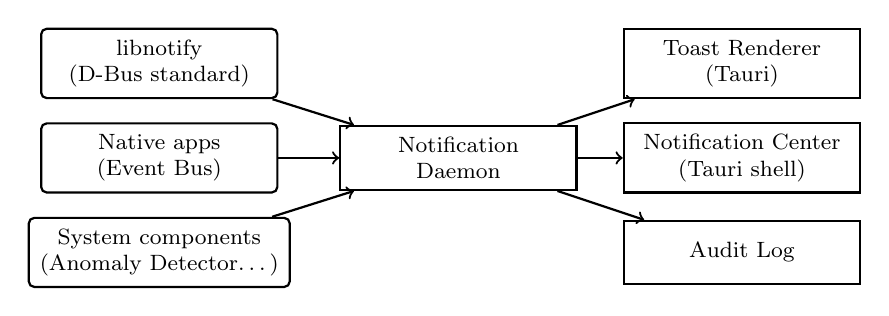
\begin{tikzpicture}[
  src/.style={
    draw, thick, rectangle, rounded corners=2pt,
    minimum width=3.0cm, minimum height=0.8cm,
    font=\footnotesize, align=center, inner sep=4pt
  },
  proc/.style={
    draw, thick, rectangle,
    minimum width=3.0cm, minimum height=0.8cm,
    font=\footnotesize, align=center, inner sep=4pt
  },
  store/.style={
    draw, thick, cylinder, shape border rotate=90,
    minimum width=1.8cm, minimum height=0.8cm,
    font=\footnotesize, align=center, inner sep=4pt
  },
  arr/.style={->, thick},
]

\node[src]  (dbus)   at (0,  2.4) {libnotify\\(D-Bus standard)};
\node[src]  (native) at (0,  1.2) {Native apps\\(Event Bus)};
\node[src]  (system) at (0,  0.0) {System components\\(Anomaly Detector\ldots)};

\node[proc] (nd)     at (3.8, 1.2) {Notification\\Daemon};

\node[proc]  (toast) at (7.4,  2.4) {Toast Renderer\\(Tauri)};
\node[proc]  (nc)    at (7.4,  1.2) {Notification Center\\(Tauri shell)};
\node[proc] (al) at (7.4, 0.0) {Audit Log};

\draw[arr] (dbus)   -- (nd);
\draw[arr] (native) -- (nd);
\draw[arr] (system) -- (nd);
\draw[arr] (nd)     -- (toast);
\draw[arr] (nd)     -- (nc);
\draw[arr] (nd)     -- (al);

\end{tikzpicture}
\caption{Notification pipeline. All sources converge on the Notification Daemon,
which normalizes, groups, and applies priority logic before forwarding to the
toast renderer and notification center. Every notification is logged in the
Audit Log by sender and timestamp, never by content.}
\label{fig:notifications}
\end{figure}

The daemon receives from two sources: the standard D-Bus interface at
\texttt{org.freedesktop.Notifications}, which means every third-party
application using \texttt{libnotify} or \texttt{notify-send} works without
changes; and the Event Bus, through which native system components send richer
notifications with priority metadata and graph context. Both are normalized to
a common internal schema before any further processing.

\begin{table}[htbp]
\caption{Notification priority levels}
\label{tab:notifications}
\begin{tabularx}{\linewidth}{lXX}
\toprule
\textbf{Level} & \textbf{Behavior} & \textbf{Do Not Disturb} \\
\midrule
Critical & Persistent toast, no auto-close &
  Always shown, never silenced \\
High     & Toast auto-closes after approximately 8 seconds &
  Delayed, not blocked \\
Normal   & Toast auto-closes after approximately 4 seconds &
  Silenced \\
Low      & No toast; goes silently to Notification Center only &
  Silenced \\
\bottomrule
\end{tabularx}
\end{table}

Critical priority is reserved for system-level alerts only: Anomaly Detector
warnings, component compatibility failures, and security events. Applications
cannot self-assign Critical. Notifications from the same application are
grouped in the Notification Center; as a toast, only the most recent
notification from an application is shown, with a counter if a previous one
from the same application is still visible. Do Not Disturb has three modes
(off, on, and scheduled by time of day) and is togglable from the taskbar quick
panel.

Focus Mode (Section~\ref{sec:focus-mode}) interacts with the notification
priority system directly. When a project declares a \texttt{[focus]} block
with \texttt{suppress\_notifications\_from}, the daemon demotes matching
application notifications to Low priority for the duration of the focused
session. This demotion is applied by the daemon at routing time, not by
modifying the application's permanent permission profile. Critical-priority
alerts from system components are exempt and always pass through regardless
of Focus Mode state.

\subsection{Permission System}
\label{sec:permissions}

Every application on the system, whether a first-party app, a Flatpak, or an
RPM package, operates within a permission profile that defines what it can
access. The system is unified: one file format, one enforcement layer, one
place for the user to review and adjust everything.

\paragraph{Permission file format.}
Each application has a TOML permission file at
\texttt{\textasciitilde/.config/permissions/<app-id>.toml} that serves as the
sole source of truth for what that application is allowed to do. The file is
human-readable and user-editable; the Settings app provides a UI for those who
prefer not to edit it directly. Permissions are enforced via Linux namespaces,
AppArmor, and seccomp, described in Section~\ref{sec:security}.

\begin{lstlisting}[language=bash, caption={Example permission file}]
# ~/.config/permissions/org.mozilla.firefox.toml

[filesystem]
allow = ["~/Downloads", "~/Documents", "~/.mozilla"]

[network]
allow = ["full"]

[devices]
allow = ["gpu"]

[graph]
# no entry = no access, never prompted
\end{lstlisting}

Graph access is never inferred or learned. An application with no
\texttt{[graph]} section has no graph access, with no exceptions and no
automatic prompting. Graph permissions must be explicitly declared.

\paragraph{Store-supplied profiles.}
The Store ships a curated permission profile alongside known applications.
Common software such as Firefox, LibreOffice, and VLC has community-maintained
profiles that are installed automatically and shown to the user at install time
for review. Community members can submit profiles for applications not yet
covered; submitted profiles go through Store review before publication, since
an overly permissive profile is a meaningful risk. Permission profiles are one
component of the broader Integration Package system described in
Section~\ref{sec:integration-packages}.

\paragraph{Flatpak adapter.}
Flatpak applications carry their own permission declarations. When a Flatpak is
installed, the system automatically generates a native permission file by
mapping Flatpak permissions to the native format: \texttt{filesystem=home}
becomes \texttt{filesystem.allow = ["\textasciitilde/"]}, and so on. The
generated file is shown to the user at install time and can be tightened before
confirming. The Flatpak manifest is the floor; the system never grants more
than what the Flatpak declared.

\paragraph{First-run learning mode.}
If no Store profile exists and the application is not a Flatpak, the first
launch runs in learning mode: all accesses are permitted and logged, nothing is
blocked. The learning window closes automatically ten minutes after first
launch, or when the session ends, whichever comes first. The user then receives
a summary of what the application accessed, with options to review and confirm,
edit first, or start with all permissions blocked. From the second launch
onward, the confirmed profile is enforced. Learning mode applies to filesystem,
network, and device access only; graph access is always denied until explicitly
granted and cannot be learned. During the learning window, at most five new
permission grants are recorded per minute; exceeding this rate suspends
learning immediately and generates an anomaly alert. This limits the damage
from a compromised application that attempts to accumulate permissions in bulk
during its first session.

\paragraph{Runtime behavior.}
When an application attempts an access outside its profile, the access is
denied and the user receives a notification offering to extend the profile.
If the user allows, the profile is updated and the application retries the
action; if the user denies, the block stands. Repeated denials for the same
path are collapsed: after three denials for the same access, the system asks
once whether to always block it rather than continuing to prompt.

\paragraph{Ephemeral app mode.}
Any application can be launched in ephemeral mode, either from the right-click
context menu in the launcher or via a command-line flag. Ephemeral mode
combines several existing sandbox mechanisms into a single preset with no
configuration required.

In ephemeral mode, a private Mount Namespace is created with no write access
to the home directory; the application sees a temporary overlay that is
discarded on exit. Graph access is entirely disabled regardless of the
application's normal permission profile. Network activity is permitted if
declared in the application manifest, but is not logged to the Audit Log.
On exit, the temporary overlay is deleted, no entries are written to the
Knowledge Graph, and no permission changes persist.

The intended use case is opening untrusted or one-off content: a PDF from an
unknown sender, a binary downloaded for a single use, or any application the
user wants to run without leaving a trace. Ephemeral mode is not a replacement
for the full profile isolation that separate Linux users provide; it does not
protect against a compromised application exploiting a kernel vulnerability.
What it provides is a low-friction way to reduce the footprint of routine
untrusted content without requiring a separate session or a virtual machine.

\subsection{Integration Packages}
\label{sec:integration-packages}

An Integration Package is a Store package that describes how the system
integrates with a specific third-party application. It is not a bundle: it
contains no application binaries. It is a declaration that references an
existing application and provides three optional components alongside it:
a permission profile, a Settings adapter, and native Settings registrations
for os-sdk applications.

The application itself and its Integration Package are two independent Store
entries with separate versions, separate maintainers, and separate update
cycles. A package published by Mozilla ships Firefox; an Integration Package
published by the community ships the permission profile and Settings adapter
for Firefox.

\paragraph{Package format.}
An Integration Package declares which application it targets and what it
provides:

\begin{lstlisting}[language=bash, caption={Integration Package manifest}]
[package]
id      = "community.firefox.integration"
name    = "Firefox Integration"
version = "2.1.0"
conflicts = ["community.firefox.privacy"]

[app]
# At least one identifier required; all three are optional
store_id     = "org.mozilla.firefox"
flatpak_id   = "org.mozilla.Firefox"
package_name = "firefox"

# Compatible with which app versions
compatible_with = ">=120.0, <130.0"

[includes]
permissions = "permissions.toml"   # optional
adapter     = "firefox-adapter.toml"  # optional
\end{lstlisting}

The \texttt{conflicts} field lists Integration Packages that are incompatible
with this one. When the Store detects a conflict at install time, it presents
the user with a choice rather than silently merging or overriding. If both
packages are installed simultaneously (for example via a package manager), the
Settings page for the affected application shows a conflict warning and the
permissions of the first-installed package remain active until the user
resolves the conflict.

\paragraph{Settings Adapter.}
The Settings Adapter is a declarative TOML document that describes how a
third-party application's native configuration file maps to Settings UI
elements. It contains no executable code; Settings interprets the declaration
and performs all reads and writes itself.

\begin{lstlisting}[language=bash, caption={Settings Adapter declaration}]
[adapter]
schema_version = "1.0"
write_strategy = "requires_app_closed"  # or "anytime"

[sources]
prefs = {
    path              = "~/.mozilla/firefox/*/prefs.js",
    format            = "firefox-prefs",
    instance_strategy = "last_used"  # or "all", "ask"
}

[[settings]]
key      = "browser.startup.homepage"
source   = "prefs"
label    = "Homepage"
type     = "string"
default  = "about:home"
section  = "General"
verify   = true

[[settings]]
key      = "browser.tabs.tabMinWidth"
source   = "prefs"
label    = "Minimum tab width"
type     = "integer"
min      = 50
max      = 250
default  = 76
section  = "Tabs"
readonly = false

[[settings]]
key      = "browser.cache.disk.capacity"
source   = "prefs"
label    = "Disk cache size (internal)"
type     = "integer"
section  = "Advanced"
readonly = true
\end{lstlisting}

\emph{write\_strategy} controls when Settings may write to the configuration
file. \texttt{anytime} writes immediately; \texttt{requires\_app\_closed}
disables all edit controls while the application is running and writes only
when it is not, because some applications overwrite their configuration on
exit and would discard changes made while running.

\emph{instance\_strategy} applies when the source path glob matches multiple
files. \texttt{last\_used} selects the file with the most recent modification
timestamp, appropriate for applications that maintain separate profiles.
\texttt{all} writes to every matched file simultaneously. \texttt{ask}
prompts the user once on the first opening of the Settings page and remembers
the selection.

\emph{verify} causes Settings to read the field back after writing and compare
it to the value it attempted to write. If the values do not match, Settings
displays an error rather than silently succeeding. This catches cases where an
application has renamed or removed a configuration key in a newer version.

\emph{readonly} fields are displayed but not editable. They carry a lock
indicator in the Settings UI.

The adapter supports the following configuration formats via built-in format
handlers: TOML, JSON, INI and \texttt{.conf} files, Firefox \texttt{prefs.js},
\texttt{.env} key-value files, and flat \texttt{key=value} files. Binary and
proprietary formats are not supported; the application page in Settings shows
only the Permissions section when no compatible adapter is available.

Adapter source files are restricted to paths within known user configuration
directories. An adapter cannot declare a source outside \texttt{\textasciitilde/.config/},
\texttt{\textasciitilde/.mozilla/}, \texttt{\textasciitilde/.local/}, and
similar user-owned paths. System paths are never writable through an adapter.

\paragraph{Compatibility and updates.}
The \texttt{compatible\_with} field declares which application versions the
Integration Package supports. When the application updates beyond the declared
range, Settings displays a compatibility warning on the application page with
a direct link to the Store listing of the Integration Package. The adapter
remains active -- most configuration keys do not change between application
versions -- but the warning signals that the package maintainer should review
and update the package.

Integration Package updates are independent of application updates. The Install
Daemon (Section~\ref{sec:install-daemon}) monitors both streams and keeps
them consistent.

\paragraph{Native app Settings registration.}
First-party applications built with os-sdk do not use the adapter mechanism.
They register their Settings interface directly at startup via os-sdk, using
the same TOML configuration system the application already uses internally.
There is no configuration file bridge and no format handler involved:

\begin{lstlisting}[language=bash, caption={Native Settings registration via os-sdk (TypeScript)}]
shell.settings.register({
  sections: [
    {
      label: "General",
      items: [
        {
          key:     "startup.restore_session",
          label:   "Restore last session on startup",
          type:    "boolean",
          default: true,
        },
        {
          key:     "editor.font_size",
          label:   "Font size",
          type:    "integer",
          min:     8,
          max:     32,
          default: 14,
        },
        {
          key:     "editor.theme",
          label:   "Editor color scheme",
          type:    "enum",
          options: ["system", "dark", "light"],
          default: "system",
        },
      ]
    }
  ]
})
\end{lstlisting}

Settings reads this registration and renders the application's configuration
section automatically. Values are read from and written to the application's
own \texttt{\textasciitilde/.config/<app-id>/config.toml} via the os-sdk
configuration system. The application observes changes via the same inotify
mechanism all other components use. No adapter, no format handler, no
intermediate layer.

The distinction between the two paths is clean: the adapter is for existing
third-party applications that the system does not control; native registration
is for applications built for this platform that already use os-sdk.

\subsection{Install Daemon}
\label{sec:install-daemon}

The Install Daemon is a background service that sits as an abstraction layer
over all package managers active on the system. Its role is to ensure that
every application installation, regardless of how it was performed, results in
a consistent system state: permissions enforced, Integration Package loaded
if available, Settings page populated.

A user who types \texttt{dnf install firefox} in a terminal has the same
expectation as a user who finds Firefox in the Store: the application works,
its permissions are set to sensible defaults, and its Settings page is ready.
The Install Daemon makes that expectation true regardless of installation path.

\paragraph{Package manager coverage.}
The daemon registers hooks with all package managers it finds on the system.
For systemd-integrated package managers (dnf, Flatpak), it uses systemd unit
hooks that emit an Event Bus message after every install, update, or removal.
For non-systemd package managers (Homebrew, Nix, Cargo, pip with
\texttt{-{}-user}), it monitors known installation paths via
\texttt{inotify}:

\begin{lstlisting}[language=bash, caption={Monitored installation paths}]
~/.homebrew/        ~/.nix-profile/
~/.cargo/bin/       ~/.local/bin/
/opt/homebrew/
\end{lstlisting}

New package managers installed after first login are detected when their binary
appears in a known package manager location. From that point the daemon begins
monitoring their output paths as well.

When the daemon detects a new application it cannot associate with a known
app-ID, it takes no action. Only positively identified applications trigger
Integration Package lookup.

\paragraph{Integration Package matching.}
After detecting a new application installation, the daemon queries the Store
catalogue for Integration Packages that reference the installed app-ID via
any of the three reference fields (\texttt{store\_id}, \texttt{flatpak\_id},
\texttt{package\_name}). Matching packages are evaluated against a three-tier
rating policy:

\begin{table}[htbp]
\caption{Install Daemon Integration Package rating policy}
\label{tab:install-rating}
\begin{tabularx}{\linewidth}{lX}
\toprule
\textbf{Condition} & \textbf{Behavior} \\
\midrule
Rating $\geq$ 4.0 and installs $\geq$ 1{,}000 &
  Installed automatically. Brief notification after completion. \\
Rating 3.0--3.9 or installs $<$ 1{,}000 &
  Notification with Install button. Not automatic. \\
Rating $<$ 3.0 or installs $<$ 100 &
  Not surfaced. Available in the Store via manual search. \\
\bottomrule
\end{tabularx}
\end{table}

If only one Integration Package exists for an application and it does not
meet the automatic threshold, the minimum rating for automatic installation
is lowered to 3.5. No Integration Package is worse than a completely absent
one from a user experience perspective.

\paragraph{Dual installation handling.}
When the same application exists as both an RPM and a Flatpak, the daemon
treats them as two separate entries. Settings shows both with distinct labels
(for example ``Firefox (System)'' and ``Firefox (Flatpak)'') and separate
application pages. The user designates one as primary in Settings; the primary
installation is used for default application associations and Waypointer
suggestions.

\paragraph{Offline queue.}
When an application is installed without network access, the daemon stores a
pending lookup entry locally. The next time the network becomes available --
detected via a NetworkManager event on the Event Bus -- the daemon processes
queued entries and applies the normal matching policy. Queue entries expire
after 30 days without resolution.

\paragraph{Update compatibility.}
Application updates are never blocked by Integration Package compatibility
status. When an application updates beyond an Integration Package's declared
\texttt{compatible\_with} range, the daemon checks the Store for a newer
version of the Integration Package. If one exists it is installed
automatically. If none exists, Settings displays a compatibility warning. The
application update proceeds regardless.

\paragraph{Deinstallation.}
When an application is removed, its Integration Package is set to inactive
rather than uninstalled. It remains visible in a dedicated ``Inactive
Integrations'' section of Settings. If the application is reinstalled, the
Integration Package reactivates automatically without prompting. Explicit
removal of the Integration Package is a separate user action available from
the inactive list or the Store.

\paragraph{Audit log.}
Every Install Daemon action is recorded in the Audit Log via the Audit Daemon:
automatic Integration Package installations, manual installations triggered by
notification, deactivations, reactivations, and failed queue resolutions. Each
entry carries the app-ID, Integration Package ID and version, trigger source,
rating and install count at decision time, and whether the action was automatic
or user-initiated.

The system is extensible at multiple layers through a unified module mechanism.
All module types use the same installation channel (the Store) and the same
manifest format, but they operate as independent subsystems with separate APIs.
A single Store package can bundle multiple module types together.

\paragraph{Module categories.}
Table~\ref{tab:modules} lists the available extension points. Theme modules
are a special case: they consist of CSS and token overrides only, contain no
executable code, and require no sandbox. All other categories run sandboxed
with declared permissions.

\begin{table}[htbp]
\caption{Module categories and extension points}
\label{tab:modules}
\begin{tabularx}{\linewidth}{llX}
\toprule
\textbf{Category} & \textbf{Extension point} & \textbf{Example} \\
\midrule
\texttt{theme}               & Design language layer     & Community color schemes \\
\texttt{waypointer.provider} & Waypointer search results & Web search, stock prices \\
\texttt{waypointer.action}   & Waypointer command actions & Create task, send message \\
\texttt{shell.topbar}        & Topbar element slot       & Custom status widget \\
\texttt{shell.widget}        & Desktop widget area       & Clock, weather, system stats \\
\texttt{mcp.server}          & AI MCP integration        & External service connector \\
\texttt{keybinding.profile}  & Global input manager      & Alternative layout profiles \\
\bottomrule
\end{tabularx}
\end{table}

\paragraph{Manifest format.}
Every module package has a single manifest that declares what it provides,
its dependencies, conflicts, and permissions. The \texttt{[permissions]} block
uses the same schema as application permission files; at install time the
Module Runtime generates the permission file from the manifest and the user can
inspect and adjust it in Settings like any other application.

\begin{lstlisting}[language=bash, caption={Example module manifest}]
[package]
id      = "com.example.ai-waypointer"
name    = "AI Waypointer Provider"
version = "1.0.0"

[provides]
waypointer.provider = true

[activation]
# Optional: only run this module when a focused project carries these tags.
# The Module Runtime starts and stops the module as Focus Mode changes.
# Omit this block for modules that run unconditionally.
active_when_focused = { require_tags = ["rust"] }

[dependencies]
shell   = ">=1.2"
modules = ["com.example.ai-core"]

[permissions]
network.allow = ["api.openai.com"]
graph.allow   = ["read"]
\end{lstlisting}

The \texttt{[activation]} block is optional. When present, the Module Runtime
evaluates it against the active \texttt{Project} node each time Focus Mode
changes. A module with \texttt{require\_tags = ["rust"]} is started when the
focused project carries the \texttt{rust} tag and stopped when Focus Mode
deactivates or switches to a project that does not. The module's declared
permissions apply for the duration it is running; they are not expanded or
restricted by the activation condition. A module started via project activation
follows the same crash recovery policy as any other module.

Modules cannot declare permissions beyond what the manifest specifies, and
manifests are reviewed during Store submission. Unlike applications, modules
cannot expand their permissions at runtime through a learning mode; their
profile is set at install time and any undeclared access returns
\texttt{EACCES}.

\paragraph{Module Runtime.}
A dedicated Module Runtime daemon manages lifecycle, sandboxing, and crash
recovery for all active modules. Each module runs in its own isolated WebView
context, separate from the shell's WebView. A module crash does not affect the
shell or other modules.

The runtime uses exponential backoff per module instance for crash recovery,
shown in Table~\ref{tab:crash-recovery}. The 60-second window resets on a
clean run, so a module that runs for several minutes and then crashes once
gets an immediate restart.

\begin{table}[htbp]
\caption{Module crash recovery policy}
\label{tab:crash-recovery}
\begin{tabularx}{\linewidth}{lX}
\toprule
\textbf{Crash count (within 60 s)} & \textbf{Behavior} \\
\midrule
1st & Immediate restart \\
2nd & Restart after 5 seconds \\
3rd & Restart after 30 seconds \\
4th or more & Marked as failed; no further automatic retries \\
\bottomrule
\end{tabularx}
\end{table}

When a module is marked failed, Settings shows a subtle error indicator with
the last crash log. The user can trigger a manual retry at any time. There is
no notification spam.

Module updates are downloaded in the background and applied at different points
depending on category: theme updates apply immediately as a token and CSS swap;
Waypointer modules update on the next Waypointer open; shell widgets and topbar
modules update on the next session start by default, with a manual
``Restart now'' option available in Settings; MCP server modules update on the
next session start to avoid interrupting active AI interactions.

\paragraph{Shell API.}
Modules interact with the system through a restricted TypeScript SDK. No direct
access to the compositor or Graph Daemon is available; what is not in
the SDK is not accessible.

\begin{lstlisting}[language=bash, caption={Module SDK surface (TypeScript)}]
import { shell } from "@os/module-sdk"

// Window management
const windows = await shell.getWindows()
const active  = await shell.getActiveWindow()

// Graph (requires graph = "read" in manifest)
const recent = await shell.graph.query(
  "MATCH (f:File) RETURN f LIMIT 5"
)

// Waypointer provider registration
shell.waypointer.register({
  id:          "com.example.ai-waypointer",
  placeholder: "Ask AI...",
  onQuery:     async (q) => [ /* result objects */ ]
})

// Focus Mode: react to project context changes
shell.focus.onActivate((project) => {
  // project.name, project.tags, project.rootPath available
})
shell.focus.onDeactivate(() => { /* cleanup */ })
\end{lstlisting}

The \texttt{shell.focus} API allows modules to react to Focus Mode transitions
without polling. A Waypointer provider that wants to narrow its result set to
the active project subscribes to \texttt{onActivate} and adjusts its query
scope accordingly; \texttt{onDeactivate} signals that the module should return
to its default behavior. These callbacks fire after all system-level Focus Mode
changes have been applied, so the project context is already consistent when
the module receives the event.

\paragraph{Global Input Manager.}
Keybindings and gestures are configured in a single place in Settings, not per
application or per module. Modules register named actions with default
bindings; the user overrides them centrally. The module never receives the
binding string directly; the Input Manager calls the registered action handler
when the binding fires. This means a user can rebind everything from one place
and no module can silently capture input outside its declared actions.

\paragraph{Developer experience.}
A CLI scaffolds a complete module project with one command:
\texttt{npx create-os-module <n>}, producing a Vite, TypeScript, Tailwind,
and module-sdk setup with a manifest template. In dev mode, the module runs
unsigned in a dedicated dev sandbox, all declared permissions are granted
without Store review, WebView DevTools are accessible, and hot-reload via Vite
is active. Dev mode is only available on developer builds; production builds
reject unsigned modules.

For distributing a finished module outside the Store, a developer generates a
self-signed key pair with the CLI, signs the module, and distributes it as an
\texttt{.osmod} file. Installation uses TOFU: the first install prompts the
user to trust the key fingerprint; subsequent updates from the same key are
silent. Sideloaded modules receive no expanded permissions and are marked
``Not from Store'' in Settings.

\subsection{Store}
\label{sec:store}

The Store is the primary distribution channel for applications, themes,
modules, and profile packages. It is designed to be financially sustainable for
the project without becoming a gatekeeper for the ecosystem.

\paragraph{Publishing.}
Publishing an application to the Store is free and remains free indefinitely.
There is no annual developer fee. Every upload runs automated technical checks:
valid permission declarations, correct package signing, sandbox policy
compatibility, and resolvable declared dependencies. These checks are
automated; no manual review is required for packages that pass them. A failed
check returns a specific error. A manual Security Review is available
optionally and is the basis for the Security Audit Badge described below.

\paragraph{Revenue model.}
Supported pricing models include free, one-time purchase, subscription,
in-app purchases, pay-what-you-want, and freemium. Developers can also direct
users to external payment links; the Store payment infrastructure is a
convenience, not a monopoly.

Commission is calculated on total annual revenue across all applications in a
developer account, using the tiered structure in Table~\ref{tab:commission}.
When a threshold is crossed mid-year, the new rate applies to all subsequent
transactions in that year, not retroactively.

\begin{table}[htbp]
\caption{Store commission tiers}
\label{tab:commission}
\begin{tabularx}{\linewidth}{XX}
\toprule
\textbf{Annual revenue (account total)} & \textbf{Commission} \\
\midrule
Up to \EUR{10,000}                        & 0\% \\
\EUR{10,000} to \EUR{50,000}              & 5\% \\
\EUR{50,000} to \EUR{500,000}             & 15\% \\
\EUR{500,000} to \EUR{5,000,000}          & 20\% \\
Over \EUR{5,000,000}                      & 25\% \\
\bottomrule
\end{tabularx}
\end{table}

\paragraph{User-facing features.}
Purchases are tied to the user account, not the device. Trials are declared in
the app manifest and enforced by the Store; no credit card is required to start
a trial, and when it ends the user receives a single notification with a
purchase option and no automatic charges. Family Sharing is opt-in per
application: developers can allow up to six to eight family members to use an
application under one purchase. Every application's Store page shows a full
price history including every price change with its date; this is automatic and
cannot be disabled by the developer. All active subscriptions across all
applications are visible and cancellable in one place in Settings.

\paragraph{Developer dashboard.}
Developers see install counts, active user numbers, revenue and payout history,
ratings and written reviews, crash reports from users who opted into crash
reporting at the system level, and version adoption numbers. All data is
aggregated and anonymized; the developer sees counts, never identities. No
third-party analytics are required or supported.

\paragraph{Security Audit Badge.}
Applications can display a Security Audit badge on their Store page by
uploading an independent security audit report. The Store verifies that the
report originates from the stated auditing organization and links it from the
application page. Users can read the full report and judge the auditing
organization's credibility themselves. The badge means an audit exists and is
accessible, not that the Store has endorsed the application's security.

\paragraph{Long-term support.}
Developers can declare a Long Term Support commitment in the application
manifest by setting a support end date. The Store displays this date publicly
on the application page. It is a voluntary public commitment with no automated
enforcement, but the public visibility creates accountability. LTS applications
are filterable in Store search for users who prioritize stability.

\paragraph{Profile package distribution.}
Signed environment profile packages (\texttt{.lenv} files, described in
Section~\ref{sec:platform}) are distributed through the Store using the same
infrastructure as applications. Profile packages are free to publish and carry
no commission.

\paragraph{Integration Package distribution.}
Integration Packages (described in Section~\ref{sec:integration-packages}) are
distributed through the Store as a distinct package type. They are free to
publish and carry no commission. Publishing runs the same automated technical
checks as applications: valid signing, resolvable app references, and schema
validation of any included adapter declaration. A manual Security Review is
available and recommended for packages that include permission profiles, since
an overly permissive profile represents a meaningful risk.

Store listings for Integration Packages display the target application, the
package components included (permissions, adapter, or both), the
\texttt{compatible\_with} version range, and the standard rating and install
count. The Install Daemon uses rating and install count to determine automatic
installation eligibility as described in Section~\ref{sec:install-daemon}.

Deep links between Integration Package Store listings and the corresponding
application page in Settings use the \texttt{store://} and \texttt{settings://}
URL schemas described in Section~\ref{sec:settings-deeplinks}.
